\chapter{Introduction}


\section{Dataset Shift}

In the field of machine learning and predictive modeling, it is often assumed that data distributions remain static, meaning they do not change between the training and deployment phases of the model.

However, in practice, this assumption is rarely satisfied: data distributions can undergo significant changes between the training and testing scenarios.
	
\vspace{0.3cm}
	This phenomenon is known as "dataset shift" and is closely related to another field of study, referred to by various terms such as "transfer learning" or "inductive transfer".
    
    Transfer learning addresses the problem of how information can be drawn from a number of only partially related training scenarios and used to provide better predictions in one of those scenarios compared to using only that specific scenario.
    
    Therefore, dataset shift represents a more specific case: it deals with relating information in, typically, two closely related environments to improve prediction in one given the dataset in the other.
	
\vspace{0.3cm}
	Given this issue, it is crucial to develop an understanding of the suitability of particular models under such changing conditions, and it is necessary to consider whether a different predictive model should be employed.
	
\vspace{0.3cm}
	Among the various forms of dataset shift, covariate shift, studied and described by Shimodaira in 2000, is one of the most extensively researched forms.
    
    It encompasses situations where the distribution of the covariates, $P(X)$ changes, while the conditional relationship $P(Y \mid X)$, representing the relationship between the covariates $X$ and the target $Y$, remains unchanged.
    
    In this case, the typical values of the covariates observed during testing differ from those observed during training.
	
	
\subsection{Most common causes of dataset shift}
	
The two most common and studied causes of dataset shift are:

\begin{enumerate}
	\item Sample selection bias
	\item Non-stationary environments
\end{enumerate}


Sample selection bias occurs when there is a discrepancy in the data distribution due to the training data being obtained through a biased method, and therefore not reliably representing the real environment in which the classifier will be used (the test set).

It is not a flaw of an algorithm or data management but a systematic defect in the process of collecting or labeling data, which causes a non-uniform selection of training examples from a population, leading to the formation of bias during training.

Dataset shift resulting from sample selection bias is particularly relevant when dealing with imbalanced classification problems, as in highly imbalanced domains, the minority class is especially sensitive to single classification errors due to its typically low number of samples.

In real-world applications, it is often the case that data is not stationary (in time or space). One of the most relevant non-stationary scenarios involves adversarial classification problems, such as spam filtering and network intrusion detection.
	

\section{Covariate Shift}

As previously mentioned, covariate shift is a specific type of dataset shift often encountered in machine learning.
	
It occurs when the distribution of input data changes between the training environment and the operational environment, but there is no change in the underlying relationship between the input and output.  
	
Mathematically, this case can be defined as follows:  
	
	\vspace{0.5cm}  
	\textbf{Definition:} \textit{Covariate shift} occurs only in problems of the type \(X \to Y\) and is defined as the case where:  
	\[
	P_{\text{tra}}(Y \mid X) = P_{\text{tst}}(Y \mid X) \quad \text{and} \quad P_{\text{tra}}(X) \neq P_{\text{tst}}(X)
	\]
	where \(P_{\text{tra}}\) and \(P_{\text{tst}}\) represent the probability distributions in the training data and test data, respectively.  
	\vspace{0.5cm}  
	
Covariate shift is a phenomenon that can affect a wide range of machine learning models, regardless of the task they are designed to perform.

It is commonly encountered in scenarios where models classify data or predict trends based on input features.

This issue is particularly relevant in diverse machine learning applications, including but not limited to:
	
	\begin{enumerate}
		\item Image categorization and facial recognition systems
		\item Speech recognition and translation software
		\item Diagnostic and screening tools in healthcare
	\end{enumerate}
	
For example consider a model designed to distinguish between cats and dogs. Our training data might consist of images like those shown in Figure \ref{cani-gatti-tr}, present in a specific dataset.
	
	\vspace{1cm}
	\begin{figure}[h!]
		\centering
		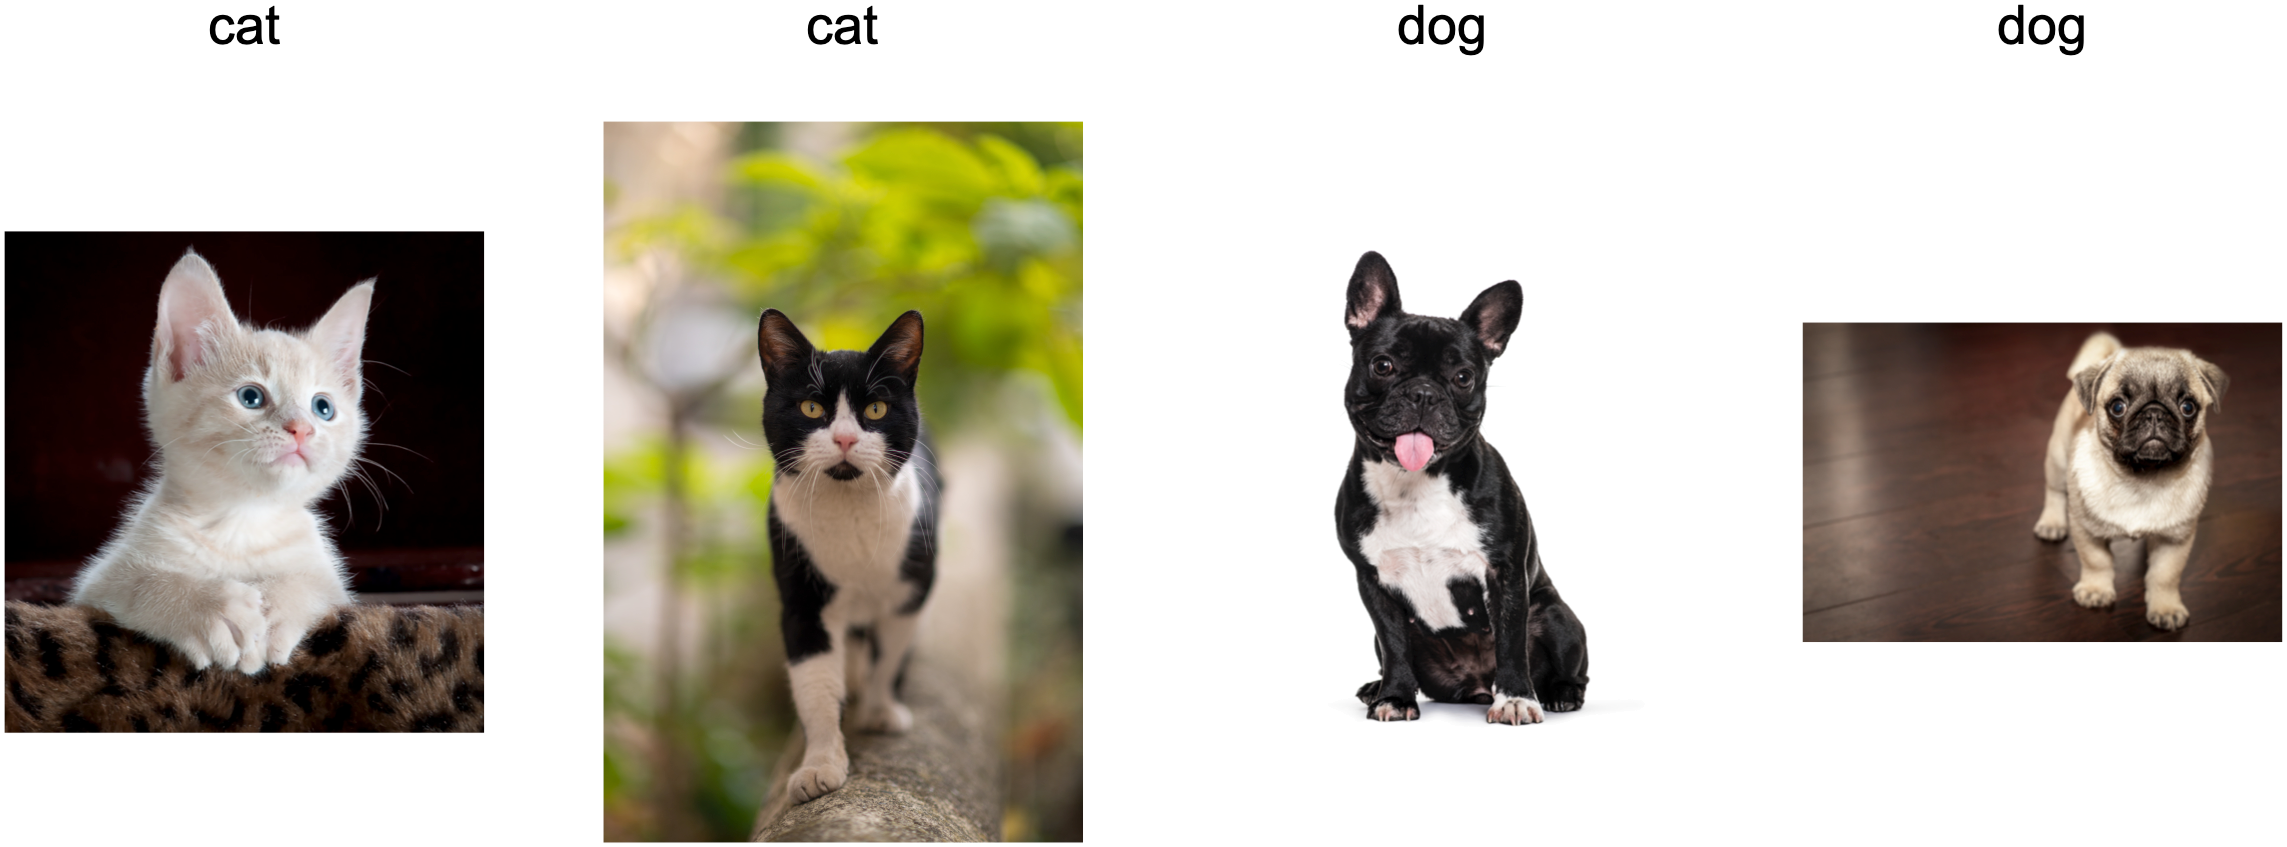
\includegraphics[width=1\textwidth]{cat-dog-train.png} 
		\caption{Training data for distinguishing cats and dogs.}
		\label{cani-gatti-tr}
	\end{figure}
     \vspace{1cm}
     

At test time, we are asked to classify the images in Figure \ref{cani-gatti-ts}. Once deployed, the model will not accurately distinguish between cats and dogs because the feature distribution will differ.

Model may achieve a high degree of accuracy on a labeled training dataset, identifying and classifying the object in an image. 

However, when deployed with real-time data, changes in the input distribution can significantly impact the model's accuracy.
		
	\vspace{1cm}
	\begin{figure}[h!]
		\centering
		
\includegraphics[width=1\textwidth]{cat-dog-test.png} 
		\caption{Test data for distinguishing cats and dogs.}
		\label{cani-gatti-ts}
	\end{figure}
	\vspace{1cm}
	
The same can be accured in the case of facial recognition. The training data might not include subjects from specific ethnicities or age groups.

When the model is deployed in a real-world environment, subjects that do not align with the training data may exhibit an unrecognizable feature distribution. 

Another cause of covariate shift could be variations in environmental conditions, such as lighting.

For instance, an image categorization model trained under specific lighting conditions may perform poorly when deployed in an operational setting with different lighting.
	
	\vspace{0.5cm}
	
So covariate shift, also known as covariate drift, is a very common issue in machine learning. Supervised learning models are often trained with labeled data. 

A data scientist typically prepares and labels the training data, identifying and analyzing outliers to maintain a high level of data quality.

However, the same level of oversight cannot be guaranteed in an operational environment since professionals will not have direct control over the input data once the model is deployed.

This means that the availability and quantity of training data can be limited, and consequently, the distribution of input data in this subset of training data is unlikely to exactly mirror the characteristics of data in a real-world environment.

Figure \ref{covariate-shift} shows an example of different distribution between training data and test data, creating a division between the two datasets.  
	

	\begin{figure}[h!]
		\centering
		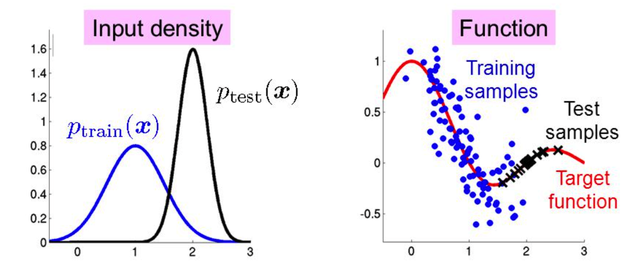
\includegraphics[width=0.8\textwidth]{immagine.png} 
		\caption{Example of covariate shift.}
		\label{covariate-shift}
	\end{figure}

	
This will have a negative impact on the accuracy of the model, as the algorithms will have been trained to map input data to output data and may fail to recognize the features of inputs from a different distribution, as shown in Figure \ref{inaccurate-model}.  
	

	\begin{figure}[h!]
		\centering
		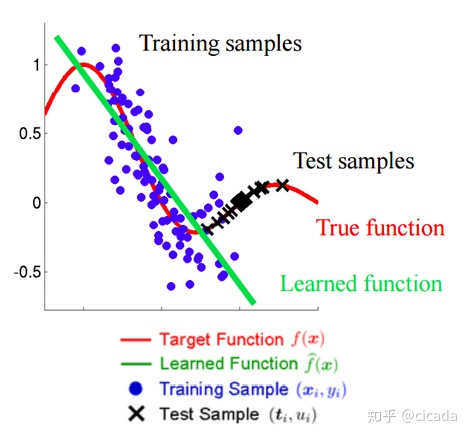
\includegraphics[width=0.5\textwidth]{covariate_shift.png} 
		\caption{Example of inaccurate model.}
		\label{inaccurate-model}
	\end{figure}  

\vspace{0.5cm}

This means that the model may become less accurate or completely ineffective. This issue represents a critical aspect in machine learning, as a highly performant model on training data may not remain accurate once deployed.

The goal is to determine the extent to which the shift affects the model, take measures to address the issues, and improve the model's accuracy.
	
Addressing this issue allows models to be readjusted to improve their accuracy. Covariate shift can provide insights into the degree of generalization of the model, which refers to the model's ability to apply learned features from training data to new data.

Low levels of generalization can result from overfitting, where the model is overly aligned with the training data, making it ineffective when encountering new data with a different distribution.  
	
	